\documentclass[tikz,border=8pt]{standalone}
\usepackage{ctex}
\usepackage{amsmath,amssymb}
\usetikzlibrary{arrows.meta,calc,angles,quotes,patterns,positioning,decorations.pathmorphing}
\definecolor{ink}{RGB}{30,43,58}
\definecolor{blue}{RGB}{38,92,168}
\definecolor{orange}{RGB}{220,112,24}
\definecolor{green}{RGB}{38,139,93}
\definecolor{red}{RGB}{192,53,53}
\definecolor{water}{RGB}{128,190,220}
\tikzset{
 line cap=round,line join=round,
 body/.style={draw=ink,very thick},
 axis/.style={-{Latex[length=2.5mm]},draw=ink,very thick},
 vec/.style={-{Latex[length=2.5mm]},draw=blue,very thick},
 force/.style={-{Latex[length=2.5mm]},draw=red,very thick},
 guide/.style={draw=ink!48,dashed},
 dim/.style={{Latex[length=2mm]}-{Latex[length=2mm]},draw=ink!70},
 ray/.style={-{Latex[length=2.2mm]},draw=orange,very thick}
}

\usetikzlibrary{decorations.pathmorphing}
\tikzset{mass/.style={circle,draw,fill=white,minimum size=7mm},curve/.style={very thick,blue},rope/.style={very thick,blue},ray/.style={very thick,blue,-{Latex}},impulse/.style={very thick,orange,-{Latex}},current/.style={very thick,orange,-{Latex}},resistor/.style={thick,decorate,decoration={zigzag,segment length=3mm,amplitude=1mm}}}
\begin{document}
% 1 question-01
\begin{tikzpicture}[x=1cm,y=1cm,font=\small]
\begin{scope}[xshift=-3cm]\draw[body,fill=blue!8] (0,0) circle(.8);\draw[guide] (0,0) circle(2);\fill (0,0) circle(2pt);\fill[orange] (2,0) circle(3pt);\draw[dim] (0,.2)--(2,.2) node[midway,above] {$r$};\node at (0,-2.6) {地月两体相对圆轨道};\end{scope}\begin{scope}[xshift=3.4cm]\draw[body,fill=blue!8] (-2,-.5) rectangle(2,.5);\draw[axis] (-2.5,0)--(2.5,0) node[right] {柱轴};\fill[orange] (0,1.8) circle(3pt) node[right] {月球};\draw[dim] (0,0)--(0,1.8) node[midway,right] {$r$};\draw[vec] (0,1.8)--(0,.8) node[left] {$g$};\node at (0,-1.3) {$v=\sqrt{2\pi G\rho R^2}$};\end{scope}
\end{tikzpicture}

% 2 solution-01
\begin{tikzpicture}[scale=.95]
 \begin{scope}[xshift=-3.5cm]
  \fill[blue!12] (0,0) circle(.9); \draw[body] (0,0) circle(.9);
  \draw[blue,very thick] (0,0) circle(2.0);
  \foreach \a in {0,45,...,315}{\draw[vec] ({1.65*cos(\a)},{1.65*sin(\a)})--({1.05*cos(\a)},{1.05*sin(\a)});}
  \node[blue] at (0,2.35) {球形高斯面};
  \node[align=center] at (0,-2.65) {$g\,4\pi r^2=4\pi GM$\\$g=GM/r^2$};
 \end{scope}
 \begin{scope}[xshift=3.2cm]
  \draw[fill=blue!8,body] (-2,-.55) rectangle (2,.55);
  \draw[green,very thick] (-2,-1.45)--(2,-1.45);
  \draw[green,very thick] (-2,1.45)--(2,1.45);
  \draw[green,very thick] (-2,0) ellipse(.32 and 1.45);
  \draw[green,very thick] (2,0) ellipse(.32 and 1.45);
  \foreach \x in {-1.5,-.6,.6,1.5}{
   \draw[vec] (\x,1.4)--(\x,.8); \draw[vec] (\x,-1.4)--(\x,-.8);}
  \node[green] at (0,1.85) {柱形高斯面};
  \node[align=center] at (0,-2.25) {$g(2\pi rL)=4\pi G\lambda L$\\$v^2=2\pi G\rho R^2$};
 \end{scope}
\end{tikzpicture}

% 3 question-02
\begin{tikzpicture}[scale=1]
 \draw[body] (-3,-1.5) rectangle (3,2.0);
 \draw[body] (-3,-1.5)--(-3,2.0);
 \fill[blue!10] (-1.75,-.25) circle(1.25);
 \draw[body] (-1.75,-.25) circle(1.25);
 \fill[ink] (-1.75,-.25) circle(2pt) node[right] {$O$};
 \fill[red] (-1.75,-.25-.62) circle(2.8pt) node[right] {$C$};
 \draw[dim] (-1.60,-.25)--(-1.60,-.87) node[midway,right] {$h$};
 \draw[dim] (-1.75,-.25)--(-.50,-.25) node[midway,above] {$r$};
 \draw[axis] (-3.5,2.45)--(-1.2,2.45) node[right] {$a$};
 \node at (0,-1.85) {车厢地板粗糙、左壁光滑};
\end{tikzpicture}

% 4 solution-02
\begin{tikzpicture}[x=1cm,y=1cm,font=\small]

 \draw[body] (-2.8,-1.5)--(2.8,-1.5);
 \draw[body] (-2.75,-1.5)--(-2.75,2.0);
 \draw[body] (-1.5,-.25) circle(1.25);
 \fill[red] (-1.5,-.85) circle(2.5pt) node[below right] {$C$};
 \draw[force] (-1.5,-.85)--(-3.3,-.85) node[left] {$m a$};
 \draw[force] (-1.5,-.85)--(-1.5,-2.3) node[below] {$mg$};
 \draw[force] (-2.75,-.25)--(-1.2,-.25) node[right] {$N_w$};
 \draw[force] (-1.5,-1.5)--(-1.5,.1) node[above] {$N_f$};
 \draw[force] (-1.5,-1.5)--(-.15,-1.5) node[right] {$f$};
 \draw[guide] (-1.5,-.25)--(-1.5,-.85);
 \node[align=left,anchor=west] at (.45,1.25)
 {$\sum F_x=0$\\$\sum F_y=0$\\$\sum\tau_C=0$};
 \node[blue,align=left,anchor=west] at (.45,-.45)
 {$a_{\min}=\dfrac{\mu rg}{h}$\\[4pt]$\mu'_{\min}=\dfrac{h}{r}$};
\node[align=left] at (1.8,-2.8) {向左离墙后仍检查地面摩擦\\$|f|=maI_C/[I_C+m(r-h)^2]$};
\end{tikzpicture}

% 5 question-03
\begin{tikzpicture}[x=1cm,y=1cm,font=\small]
\begin{scope}[xshift=-3.8cm]\draw[axis] (-2.3,0)--(2.3,0) node[right] {$x$};\draw[axis] (0,-2.3)--(0,2.3) node[above] {$y$};\draw[orange,very thick] plot coordinates {(-1.800000,-0.000000) (-1.763636,0.065274) (-1.727273,0.125416) (-1.690909,0.181239) (-1.654545,0.233348) (-1.618182,0.282211) (-1.581818,0.328197) (-1.545455,0.371604) (-1.509091,0.412678) (-1.472727,0.451621) (-1.436364,0.488606) (-1.400000,0.523779) (-1.363636,0.557266) (-1.327273,0.589176) (-1.290909,0.619606) (-1.254545,0.648638) (-1.218182,0.676347) (-1.181818,0.702801) (-1.145455,0.728056) (-1.109091,0.752167) (-1.072727,0.775182) (-1.036364,0.797143) (-1.000000,0.818089) (-0.963636,0.838056) (-0.927273,0.857076) (-0.890909,0.875179) (-0.854545,0.892391) (-0.818182,0.908737) (-0.781818,0.924240) (-0.745455,0.938920) (-0.709091,0.952796) (-0.672727,0.965886) (-0.636364,0.978206) (-0.600000,0.989769) (-0.563636,1.000590) (-0.527273,1.010681) (-0.490909,1.020053) (-0.454545,1.028715) (-0.418182,1.036678) (-0.381818,1.043950) (-0.345455,1.050538) (-0.309091,1.056448) (-0.272727,1.061687) (-0.236364,1.066261) (-0.200000,1.070172) (-0.163636,1.073426) (-0.127273,1.076026) (-0.090909,1.077973) (-0.054545,1.079271) (-0.018182,1.079919) (0.018182,1.079919) (0.054545,1.079271) (0.090909,1.077973) (0.127273,1.076026) (0.163636,1.073426) (0.200000,1.070172) (0.236364,1.066261) (0.272727,1.061687) (0.309091,1.056448) (0.345455,1.050538) (0.381818,1.043950) (0.418182,1.036678) (0.454545,1.028715) (0.490909,1.020053) (0.527273,1.010681) (0.563636,1.000590) (0.600000,0.989769) (0.636364,0.978206) (0.672727,0.965886) (0.709091,0.952796) (0.745455,0.938920) (0.781818,0.924240) (0.818182,0.908737) (0.854545,0.892391) (0.890909,0.875179) (0.927273,0.857076) (0.963636,0.838056) (1.000000,0.818089) (1.036364,0.797143) (1.072727,0.775182) (1.109091,0.752167) (1.145455,0.728056) (1.181818,0.702801) (1.218182,0.676347) (1.254545,0.648638) (1.290909,0.619606) (1.327273,0.589176) (1.363636,0.557266) (1.400000,0.523779) (1.436364,0.488606) (1.472727,0.451621) (1.509091,0.412678) (1.545455,0.371604) (1.581818,0.328197) (1.618182,0.282211) (1.654545,0.233348) (1.690909,0.181239) (1.727273,0.125416) (1.763636,0.065274) (1.800000,-0.000000)};
\draw[orange,very thick] plot coordinates {(-1.800000,0.000000) (-1.763636,-0.065274) (-1.727273,-0.125416) (-1.690909,-0.181239) (-1.654545,-0.233348) (-1.618182,-0.282211) (-1.581818,-0.328197) (-1.545455,-0.371604) (-1.509091,-0.412678) (-1.472727,-0.451621) (-1.436364,-0.488606) (-1.400000,-0.523779) (-1.363636,-0.557266) (-1.327273,-0.589176) (-1.290909,-0.619606) (-1.254545,-0.648638) (-1.218182,-0.676347) (-1.181818,-0.702801) (-1.145455,-0.728056) (-1.109091,-0.752167) (-1.072727,-0.775182) (-1.036364,-0.797143) (-1.000000,-0.818089) (-0.963636,-0.838056) (-0.927273,-0.857076) (-0.890909,-0.875179) (-0.854545,-0.892391) (-0.818182,-0.908737) (-0.781818,-0.924240) (-0.745455,-0.938920) (-0.709091,-0.952796) (-0.672727,-0.965886) (-0.636364,-0.978206) (-0.600000,-0.989769) (-0.563636,-1.000590) (-0.527273,-1.010681) (-0.490909,-1.020053) (-0.454545,-1.028715) (-0.418182,-1.036678) (-0.381818,-1.043950) (-0.345455,-1.050538) (-0.309091,-1.056448) (-0.272727,-1.061687) (-0.236364,-1.066261) (-0.200000,-1.070172) (-0.163636,-1.073426) (-0.127273,-1.076026) (-0.090909,-1.077973) (-0.054545,-1.079271) (-0.018182,-1.079919) (0.018182,-1.079919) (0.054545,-1.079271) (0.090909,-1.077973) (0.127273,-1.076026) (0.163636,-1.073426) (0.200000,-1.070172) (0.236364,-1.066261) (0.272727,-1.061687) (0.309091,-1.056448) (0.345455,-1.050538) (0.381818,-1.043950) (0.418182,-1.036678) (0.454545,-1.028715) (0.490909,-1.020053) (0.527273,-1.010681) (0.563636,-1.000590) (0.600000,-0.989769) (0.636364,-0.978206) (0.672727,-0.965886) (0.709091,-0.952796) (0.745455,-0.938920) (0.781818,-0.924240) (0.818182,-0.908737) (0.854545,-0.892391) (0.890909,-0.875179) (0.927273,-0.857076) (0.963636,-0.838056) (1.000000,-0.818089) (1.036364,-0.797143) (1.072727,-0.775182) (1.109091,-0.752167) (1.145455,-0.728056) (1.181818,-0.702801) (1.218182,-0.676347) (1.254545,-0.648638) (1.290909,-0.619606) (1.327273,-0.589176) (1.363636,-0.557266) (1.400000,-0.523779) (1.436364,-0.488606) (1.472727,-0.451621) (1.509091,-0.412678) (1.545455,-0.371604) (1.581818,-0.328197) (1.618182,-0.282211) (1.654545,-0.233348) (1.690909,-0.181239) (1.727273,-0.125416) (1.763636,-0.065274) (1.800000,0.000000)};
\fill[red] (-1.8,0) circle(3pt) node[below] {$+\lambda$};\fill[blue] (1.8,0) circle(3pt) node[below] {$-\lambda$};\node[right] at (0,1.08) {$\eta a$};\end{scope}\begin{scope}[xshift=3.8cm]\draw[body] (0,0) circle(1.8);\draw[guide] (-3.6,0)--(3.6,0);\fill[red] (-1.8,0) circle(3pt);\fill[blue] (1.8,0) circle(3pt);\node at (0,-2.4) {边界电极，固定两极电压};\end{scope}
\end{tikzpicture}

% 6 solution-03
\begin{tikzpicture}[x=1cm,y=1cm,font=\small]
\begin{scope}[xshift=-3.8cm]\draw[axis] (-2.3,0)--(2.3,0) node[right] {$x$};\draw[axis] (0,-2.3)--(0,2.3) node[above] {$y$};\draw[orange,very thick] plot coordinates {(-1.800000,-0.000000) (-1.763636,0.065274) (-1.727273,0.125416) (-1.690909,0.181239) (-1.654545,0.233348) (-1.618182,0.282211) (-1.581818,0.328197) (-1.545455,0.371604) (-1.509091,0.412678) (-1.472727,0.451621) (-1.436364,0.488606) (-1.400000,0.523779) (-1.363636,0.557266) (-1.327273,0.589176) (-1.290909,0.619606) (-1.254545,0.648638) (-1.218182,0.676347) (-1.181818,0.702801) (-1.145455,0.728056) (-1.109091,0.752167) (-1.072727,0.775182) (-1.036364,0.797143) (-1.000000,0.818089) (-0.963636,0.838056) (-0.927273,0.857076) (-0.890909,0.875179) (-0.854545,0.892391) (-0.818182,0.908737) (-0.781818,0.924240) (-0.745455,0.938920) (-0.709091,0.952796) (-0.672727,0.965886) (-0.636364,0.978206) (-0.600000,0.989769) (-0.563636,1.000590) (-0.527273,1.010681) (-0.490909,1.020053) (-0.454545,1.028715) (-0.418182,1.036678) (-0.381818,1.043950) (-0.345455,1.050538) (-0.309091,1.056448) (-0.272727,1.061687) (-0.236364,1.066261) (-0.200000,1.070172) (-0.163636,1.073426) (-0.127273,1.076026) (-0.090909,1.077973) (-0.054545,1.079271) (-0.018182,1.079919) (0.018182,1.079919) (0.054545,1.079271) (0.090909,1.077973) (0.127273,1.076026) (0.163636,1.073426) (0.200000,1.070172) (0.236364,1.066261) (0.272727,1.061687) (0.309091,1.056448) (0.345455,1.050538) (0.381818,1.043950) (0.418182,1.036678) (0.454545,1.028715) (0.490909,1.020053) (0.527273,1.010681) (0.563636,1.000590) (0.600000,0.989769) (0.636364,0.978206) (0.672727,0.965886) (0.709091,0.952796) (0.745455,0.938920) (0.781818,0.924240) (0.818182,0.908737) (0.854545,0.892391) (0.890909,0.875179) (0.927273,0.857076) (0.963636,0.838056) (1.000000,0.818089) (1.036364,0.797143) (1.072727,0.775182) (1.109091,0.752167) (1.145455,0.728056) (1.181818,0.702801) (1.218182,0.676347) (1.254545,0.648638) (1.290909,0.619606) (1.327273,0.589176) (1.363636,0.557266) (1.400000,0.523779) (1.436364,0.488606) (1.472727,0.451621) (1.509091,0.412678) (1.545455,0.371604) (1.581818,0.328197) (1.618182,0.282211) (1.654545,0.233348) (1.690909,0.181239) (1.727273,0.125416) (1.763636,0.065274) (1.800000,-0.000000)};
\draw[orange,very thick] plot coordinates {(-1.800000,0.000000) (-1.763636,-0.065274) (-1.727273,-0.125416) (-1.690909,-0.181239) (-1.654545,-0.233348) (-1.618182,-0.282211) (-1.581818,-0.328197) (-1.545455,-0.371604) (-1.509091,-0.412678) (-1.472727,-0.451621) (-1.436364,-0.488606) (-1.400000,-0.523779) (-1.363636,-0.557266) (-1.327273,-0.589176) (-1.290909,-0.619606) (-1.254545,-0.648638) (-1.218182,-0.676347) (-1.181818,-0.702801) (-1.145455,-0.728056) (-1.109091,-0.752167) (-1.072727,-0.775182) (-1.036364,-0.797143) (-1.000000,-0.818089) (-0.963636,-0.838056) (-0.927273,-0.857076) (-0.890909,-0.875179) (-0.854545,-0.892391) (-0.818182,-0.908737) (-0.781818,-0.924240) (-0.745455,-0.938920) (-0.709091,-0.952796) (-0.672727,-0.965886) (-0.636364,-0.978206) (-0.600000,-0.989769) (-0.563636,-1.000590) (-0.527273,-1.010681) (-0.490909,-1.020053) (-0.454545,-1.028715) (-0.418182,-1.036678) (-0.381818,-1.043950) (-0.345455,-1.050538) (-0.309091,-1.056448) (-0.272727,-1.061687) (-0.236364,-1.066261) (-0.200000,-1.070172) (-0.163636,-1.073426) (-0.127273,-1.076026) (-0.090909,-1.077973) (-0.054545,-1.079271) (-0.018182,-1.079919) (0.018182,-1.079919) (0.054545,-1.079271) (0.090909,-1.077973) (0.127273,-1.076026) (0.163636,-1.073426) (0.200000,-1.070172) (0.236364,-1.066261) (0.272727,-1.061687) (0.309091,-1.056448) (0.345455,-1.050538) (0.381818,-1.043950) (0.418182,-1.036678) (0.454545,-1.028715) (0.490909,-1.020053) (0.527273,-1.010681) (0.563636,-1.000590) (0.600000,-0.989769) (0.636364,-0.978206) (0.672727,-0.965886) (0.709091,-0.952796) (0.745455,-0.938920) (0.781818,-0.924240) (0.818182,-0.908737) (0.854545,-0.892391) (0.890909,-0.875179) (0.927273,-0.857076) (0.963636,-0.838056) (1.000000,-0.818089) (1.036364,-0.797143) (1.072727,-0.775182) (1.109091,-0.752167) (1.145455,-0.728056) (1.181818,-0.702801) (1.218182,-0.676347) (1.254545,-0.648638) (1.290909,-0.619606) (1.327273,-0.589176) (1.363636,-0.557266) (1.400000,-0.523779) (1.436364,-0.488606) (1.472727,-0.451621) (1.509091,-0.412678) (1.545455,-0.371604) (1.581818,-0.328197) (1.618182,-0.282211) (1.654545,-0.233348) (1.690909,-0.181239) (1.727273,-0.125416) (1.763636,-0.065274) (1.800000,0.000000)};
\fill[red] (-1.8,0) circle(3pt) node[below] {$+\lambda$};\fill[blue] (1.8,0) circle(3pt) node[below] {$-\lambda$};\node[right] at (0,1.08) {$\eta a$};\end{scope}\begin{scope}[xshift=3.8cm]\draw[body] (0,0) circle(1.8);\draw[guide] (-3.6,0)--(3.6,0);\fill[red] (-0.9,0) circle(3pt) node[below] {$ + $};\fill[blue] (0.9,0) circle(3pt) node[below] {$ - $};\fill[red] (-3.6,0) circle(3pt) node[below] {$ + $};\fill[blue] (3.6,0) circle(3pt) node[below] {$ - $};\node at (0,2.3) {同号反演像源};\node at (0,-2.4) {$\Delta U=2A L_\mu$};\end{scope}
\end{tikzpicture}

% 7 question-04
\begin{tikzpicture}[scale=1]
 \draw[body,line width=3pt] (-3,2.2)--(-3,-1.5)--(3,-1.5)--(3,2.2);
 \draw[water,line width=8pt] (-3,.65)--(-3,-1.5)--(3,-1.5)--(3,.65);
 \draw[guide,line width=1.2pt] (-1,2.45)--(-1,-2.0);
 \node[above] at (-1,2.45) {转轴};
 \draw[dim] (-3,-2.1)--(3,-2.1) node[midway,below] {$3l$};
 \draw[dim] (-3.65,-1.5)--(-3.65,2.2) node[midway,left] {$h$};
 \draw[dim] (-3,1.65)--(-1,1.65) node[midway,above] {$l$};
 \draw[guide] (-3,.65)--(3,.65);
 \node[right] at (3,.65) {$h/2$};
\end{tikzpicture}

% 8 solution-04
\begin{tikzpicture}[scale=.95]
 \draw[body,line width=3pt] (-3,2.4)--(-3,-1.6)--(3,-1.6)--(3,2.4);
 \draw[water,line width=8pt] (-3,.35)--(-3,-1.6)--(3,-1.6)--(3,1.45);
 \draw[guide] (-1,2.65)--(-1,-1.6);
 \node[above] at (-1,2.65) {轴};
 \draw[dim] (-3,1.95)--(-1,1.95) node[midway,above] {$l$};
 \draw[dim] (-1,1.95)--(3,1.95) node[midway,above] {$2l$};
 \draw[dim] (-3.5,.9)--(-3.5,1.45) node[midway,left] {$2\Delta h$};
 \draw[vec] (-3,.35)--(-3,-.25) node[left] {$x$};
 \draw[vec] (3,1.45)--(3,2.05) node[right] {$x$};
 \draw[green,line width=5pt] (-3,-1.6)--(3,-1.6);
 \node[green,above] at (0,-1.48) {$I_{\rm bottom}=3\rho Sl^3$};
 \node[align=center] at (0,-2.65)
 {$I(x)=\rho Sl^2(A+3x)$\quad$J=I\omega=\text{常量}$};
\end{tikzpicture}

% 9 question-05
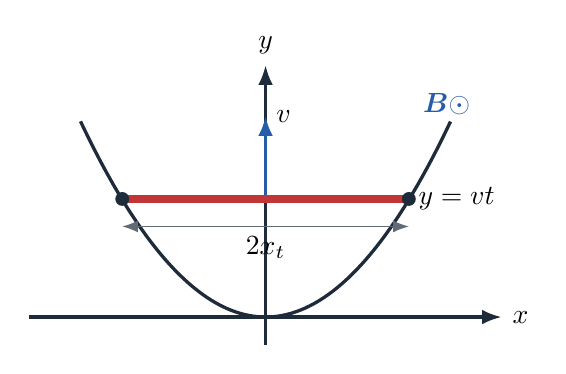
\begin{tikzpicture}[scale=1]
 \draw[axis] (-3,0)--(3,0) node[right] {$x$};
 \draw[axis] (0,-.35)--(0,3.2) node[above] {$y$};
 \draw[body,domain=-2.35:2.35,samples=80] plot (\x,{.45*\x*\x});
 \draw[red,line width=3pt] (-1.82,1.5)--(1.82,1.5);
 \fill[ink] (-1.82,1.5) circle(2.5pt); \fill[ink] (1.82,1.5) circle(2.5pt);
 \draw[vec] (0,1.55)--(0,2.55) node[right] {$v$};
 \node[right] at (1.82,1.5) {$y=vt$};
 \node[blue] at (2.3,2.7) {$\boldsymbol B\odot$};
 \draw[dim] (-1.82,1.15)--(1.82,1.15) node[midway,below] {$2x_t$};
\end{tikzpicture}

% 10 solution-05
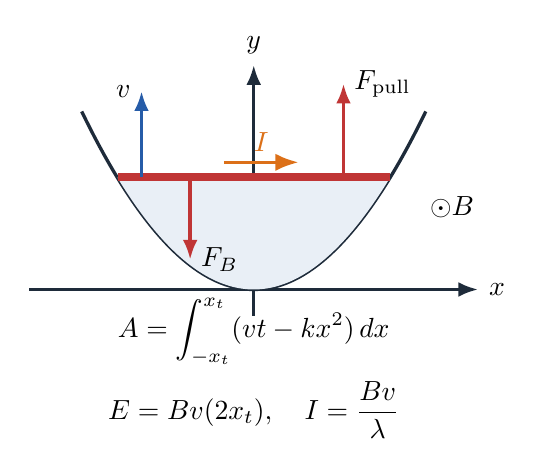
\begin{tikzpicture}[scale=.95]
 \draw[axis] (-3,0)--(3,0) node[right] {$x$};
 \draw[axis] (0,-.35)--(0,3.0) node[above] {$y$};
 \draw[body,domain=-2.3:2.3,samples=80] plot (\x,{.45*\x*\x});
 \fill[blue!10] (-1.82,1.5)--plot[domain=-1.82:1.82,samples=60] (\x,{.45*\x*\x})--cycle;
 \draw[red,line width=3pt] (-1.82,1.5)--(1.82,1.5);
 \draw[force] (-.85,1.5)--(-.85,.4) node[right] {$F_B$};
 \draw[force] (1.2,1.5)--(1.2,2.75) node[right] {$F_{\rm pull}$};
 \draw[vec] (-1.5,1.5)--(-1.5,2.65) node[left] {$v$};
 \draw[current] (-.4,1.7)--(.6,1.7) node[midway,above] {$I$};
 \node at (2.65,1.1) {$\odot B$};
 \node[align=center] at (0,-1.05)
 {$A=\displaystyle\int_{-x_t}^{x_t}(vt-kx^2)\,dx$\\[5pt]
  $E=Bv(2x_t),\quad I=\dfrac{Bv}{\lambda}$};
\end{tikzpicture}

% 11 question-06
\begin{tikzpicture}[scale=.95]
 \begin{scope}[xshift=-3.3cm]
  \draw[body,fill=orange!8] (0,0) circle(1.65);
  \fill[blue] ({1.65*cos(35)},{1.65*sin(35)}) circle(2.5pt);
  \draw[ray] ({1.65*cos(35)},{1.65*sin(35)})--++(35:2.3);
  \draw[guide] ({1.65*cos(35)},{1.65*sin(35)})--++(35:1.0);
  \node at (0,-2.05) {均匀球形余弦发光体};
 \end{scope}
 \begin{scope}[xshift=3cm]
  \draw[body] (-2.3,0)--(2.3,0);
  \draw[body,fill=blue!8] (-2,0) arc[start angle=180,end angle=0,radius=2];
  \fill[orange!25] (-2.3,-.18) rectangle (2.3,0);
  \node[below] at (0,-1.0) {余弦发光平面};
  \draw[ray] (.4,0)--(1.15,1.64)--(1.15,3.0);
  \draw[guide] (0,0)--(1.15,1.64);
  \node[right] at (1.15,2.65) {远处观察者};
  \draw[dim] (0,-.55)--(2,-.55) node[midway,below] {$r$};
 \end{scope}
\end{tikzpicture}

% 12 solution-06
\begin{tikzpicture}[x=1cm,y=1cm,font=\small]
\begin{scope}[xshift=-3.5cm]\draw[body] (-2,0) arc(180:0:2);\draw[body] (-2,0)--(2,0);\draw[guide] (0,0)--(1.414,1.414);\draw[ray] (0.7758146081336154,0)--(1.414,1.414)--(1.414,3);\node at (0,-.7) {反向光路；$i\le30^\circ$};\end{scope}\begin{scope}[xshift=1.2cm]\draw[axis] (0,0)--(4.7,0) node[right] {$a/r$};\draw[axis] (0,0)--(0,3) node[above] {$I/I_0$};\draw[blue,very thick] (0,.7)--(3.6,.7);\draw[orange,very thick] (3.6,2.6)--(4.5,2.6);\draw[guide] (3.6,0)--(3.6,2.8);\node[left] at (0,.7) {$1/4$};\node[left] at (0,2.6) {$1$};\node[below] at (3.6,0) {$1$};\node at (2.2,-1.1) {$I_0$ 指直接射入玻璃的亮度};\end{scope}
\end{tikzpicture}

% 13 question-07
\begin{tikzpicture}[x=1cm,y=1cm,font=\small]
\draw[body,fill=blue!6] (0,0) circle(2);\draw[ray] plot coordinates {(-3.018350,1.721326) (-1.018350,1.721326) (1.866975,0.717219) (0.396025,-1.960399) (-1.089572,-3.299429)};
\draw[guide] plot coordinates {(0.000000,0.000000) (-1.018350,1.721326)};
\draw[guide] plot coordinates {(0.000000,0.000000) (1.866975,0.717219)};
\draw[guide] plot coordinates {(0.000000,0.000000) (0.396025,-1.960399)};
\node at (0,-3.8) {一级虹：一次内反射，$n=4/3$};
\coordinate (O) at (0,0);
\coordinate (P) at (-1.018350,1.721326);
\coordinate (A) at (-3.018350,1.721326);
\coordinate (R) at (1.866975,0.717219);
\coordinate (N) at (-1.527525,2.581989);
\draw[guide] (P)--(N);
\pic[draw=blue,angle radius=7mm,angle eccentricity=1.4,"$\alpha$"] {angle=N--P--A};
\pic[draw=green,angle radius=9mm,angle eccentricity=1.3,"$\theta$"] {angle=O--P--R};
\end{tikzpicture}

% 14 solution-07
\begin{tikzpicture}[x=1cm,y=1cm,font=\small]
\draw[body,fill=blue!6] (0,0) circle(2);\draw[ray] plot coordinates {(-3.018350,1.721326) (-1.018350,1.721326) (1.866975,0.717219) (0.396025,-1.960399) (-1.089572,-3.299429)};
\draw[guide] plot coordinates {(0.000000,0.000000) (-1.018350,1.721326)};
\draw[guide] plot coordinates {(0.000000,0.000000) (1.866975,0.717219)};
\draw[guide] plot coordinates {(0.000000,0.000000) (0.396025,-1.960399)};
\node at (0,-3.8) {一级虹：一次内反射，$n=4/3$};\node at (0,3) {$\Delta_1=\pi+2\alpha-4\theta$；$\alpha_{1m}=59.39^\circ$};
\coordinate (O) at (0,0);
\coordinate (P) at (-1.018350,1.721326);
\coordinate (A) at (-3.018350,1.721326);
\coordinate (R) at (1.866975,0.717219);
\coordinate (N) at (-1.527525,2.581989);
\draw[guide] (P)--(N);
\pic[draw=blue,angle radius=7mm,angle eccentricity=1.4,"$\alpha$"] {angle=N--P--A};
\pic[draw=green,angle radius=9mm,angle eccentricity=1.3,"$\theta$"] {angle=O--P--R};
\end{tikzpicture}

% 15 question-08
\begin{tikzpicture}[scale=.95]
 \draw[body,fill=blue!8] (-3,-.65)--(-1.2,-.65)--(-.45,0)--(-1.2,.65)--(-3,.65)--cycle;
 \draw[force] (-3.1,.32)--(-4.4,.32);
 \draw[force] (-3.1,-.32)--(-4.4,-.32);
 \draw[force] (-.4,0)--(1.6,0) node[right] {$F$};
 \node at (-1.85,0) {飞船};
 \fill[red] (-3.6,0) circle(2pt);\fill[red] (-4.0,0) circle(2pt);
\node[red,left] at (-4.4,0) {$\mathrm{He}^{2+}$ 喷流};
 \node[align=center] at (3.35,.55)
 {$4\mathrm H^+\rightarrow\mathrm{He}^{2+}$\\$+2e^++2\nu_e+n_\gamma\gamma$};
 \node[align=center] at (3.35,-.65)
 {$m_{\rm fuel}/m_{\rm ship}=100$\\巡航固有时 $15\,\mathrm{yr}$};
\end{tikzpicture}

% 16 solution-08
\begin{tikzpicture}[scale=.9]
 \begin{scope}[xshift=-3.8cm]
  \draw[body,fill=blue!8] (-2,-.55)--(-.6,-.55)--(0,0)--(-.6,.55)--(-2,.55)--cycle;
  \draw[force] (-2.1,0)--(-4.0,0);
  \node[above,red] at (-3.1,.3) {$p_{\rm He}=\gamma_um_{\rm He}u$};
  \draw[force] (0,0)--(1.8,0) node[right] {$F$};
  \node at (-1.15,0) {飞船};
 \end{scope}
 \begin{scope}[xshift=2.2cm]
  \draw[axis] (-.2,0)--(5.7,0) node[right] {飞行阶段};
  \draw[axis] (-.2,0)--(-.2,2.2) node[above] {$v$};
  \draw[blue,line width=3pt] (.2,0)--(2.1,1.7)--(3.5,1.7)--(5.35,0);
  \node[below] at (1.15,0) {加速};
  \node[below] at (2.8,0) {巡航};
  \node[below] at (4.45,0) {减速};
  \node[above] at (2.8,1.7) {$v_c$};
  \node[blue,align=center] at (2.8,-1.45)
  {$R_{\rm acc}=R_{\rm dec}=\sqrt{101}$\\[5pt]
   $S=\sinh\!\left(\dfrac{u_{\rm eff}}{2c}\ln101\right)c\tau$};
 \end{scope}
\end{tikzpicture}

\end{document}
